% Diese Zeile bitte -nicht- aendern.
\documentclass[course=erap]{aspdoc}

%%%%%%%%%%%%%%%%%%%%%%%%%%%%%%%%%
\newcommand{\theGroup}{191} % Beispiel: 42
\newcommand{\theNumber}{A309} % Beispiel: A123
\author{Qichen Liu  \and Zhiyuan Ni \and Wenjie Zhu}
\date{Sommersemester 2021/22} % Beispiel: Wintersemester 2019/20
%%%%%%%%%%%%%%%%%%%%%%%%%%%%%%%%%

% Diese Zeile bitte -nicht- aendern.
\title{Gruppe \theGroup{} -- Abgabe zu Aufgabe \theNumber}

\begin{document}
\maketitle

\section{Einleitung}
\subsection{Schnelle Exponentiation}
Wir beschäftigen uns in der Aufgabe mit schneller Exponentiation, die auch als \glqq Binäre Exponentiation\grqq{} bekannt ist. Das Ziel dieses Verfahrens ist, bei der Berechnung eines ganzzahligen Exponenten $a^{n}$ die benötigten Multiplikationen zu reduzieren. Um das zu realisieren, ersetzt man den Exponent durch seine binäre Repräsentation.

\subsection{Aufgabenstellung}
Die gegebene Aufgabenstellung ist in einen theoretischen und einen praktischen Teil aufgeteilt. Der theoretische Teil befasst sich mit der Funktionsweise der schnellen Exponentiation und seiner Übertragung auf Matrizen, die Multiplikation zweier Zahlen beliebiger Größe sowie eine Performanzanalyse mit einer Vergleichsimplementierung. Der praktische Teil beinhaltet die Implementierung einer Berechnung für die $n$-te Fibonacci-Zahl mithilfe schneller Exponentiation. Dabei soll die C-Implementierung die folgende Funktionssignatur haben:
\begin{lstlisting}[language=C]
void fib(uint64_t n, size_t len, uint8_t buf[len]);
\end{lstlisting}
Diese Funktion nimmt das $uint64\_t$ Argument $n$ und berechnet die Fibonacci-Zahl mit diesem Index. Das Argument $buf$ ist ein Array mit dem Typ $uint8\_t$. Das zuvor berechnete Ergebnis wird dann in Little-Endian-Byte-Order in den mit $buf$ beginnenden Speicherbereich geschrieben. Das $size\_t$ Argument $len$ gibt zusätzlich in Byte ($uint8\_t$) an, wie lang dieser Speicherbereich ist, da man sonst nicht weißt, wo das Array endet. Die Allokation der entsprechenden Datenstruktur erfolgt im Rahmenprogramm. Dafür muss es vor der tatsächlichen Berechnung schon bestimmt werden, wie viel Speicherplatz die $n$-te Fibonacci-Zahl verbrauchen kann. Die Herleitung dieser Länge befindet sich im Lösungsansatz. Außerdem muss das Endergebnis im hexadezimalen Format und dezimalem Format in die Kommando-Zeile ausgegeben werden.

\subsection{Ergebnis}
Unsere Implementierung ist in der Lage, eine \glqq beliebige\grqq{} Fibonacci-Zahl zu berechnen. Mit \glqq beliebig\grqq{} ist hier gemeint, dass der Programm bis hin zum vollständigen Verbrauchen der zu Verfügung stehenden Heap-Ressourcen das richtige Ergebnis liefert. Nach unserer Erfahrung berechnet unser Programm innerhalb von 30 Minuten sogar die $400.000$-te Fibonacci-Zahl, obwohl diese Zahl in der Realität keine praktische Bedeutung hat. Als einen wichtigen Bestandteil dieser Implementierung haben wir noch eine Multiplikation mittels Karazuba-Algorithmus realisiert, welche uns erlaubt, zwei Integer beliebiger Länge miteinander zu multiplizieren. Diese Multiplikation hat den Umfang der Fibonacci-Zahl-Berechnung erheblich erweitertet und die Realisierung der Optimierung mittels schneller Exponentiation ermöglicht.

\section{Lösungsansatz}
\subsection{Theoretischer Teil}
\subsubsection{Fibonacci Matrix}
In der Aufgabe wollen wir mithilfe schneller Exponentiation die Matrix-Potenz berechnen und auf das Fallbeispiel \glqq Berechnung der Fibonacci Folge\grqq{} anwenden. Die Fibonacci Folge ist eine Reihe von Zahlen, die ab der zweiten Zahl jeweils unmittelbar aus der Summe der zwei vorherigen Zahlen bestehen
\cite{fibonacciNumbers}.
\\Betrachten wir nun das folgende Gleichungssystem\cite{fibonacciMatrix}
\begin{align*}
    f_{n+1} &= f_n + f_{n-1} \\
    f_n &= f_n
\end{align*}
und seine Schreibweise in Matrix:
\[\begin{pmatrix} f_{n+1} \\ f_n \end{pmatrix} = \begin{pmatrix} 1 &1 \\ 1 &0 \end{pmatrix} \begin{pmatrix} f_n \\ f_{n-1} \end{pmatrix} \]
Wir definieren zusätzlich $f_{-1} := 1$. Setzt man $F_n := \begin{pmatrix} f_n \\ f_{n-1} \end{pmatrix}$ und $A := \begin{pmatrix} 1 &1 \\ 1 &0 \end{pmatrix}$ ein,
so erhält man $F_{n+1} = AF_n$. Darauf basierend ist es einfach zu zeigen, dass $F_n = AF{n-1}$ gilt. Man setzt diese Gleichung für $F_n$ ein und durch vollständige Induktion erhält man
\begin{equation*}
    F_{n+1} = A^nF_1
    \text{ und }
    F_n = A^nF_0
\end{equation*}
Die beiden Spaltenvektoren $F_{n+1}$ und $F_n$ kann man zu einer 2 $\times$ 2-Matrix
\[(F_{n+1} \; F_n) = \begin{pmatrix} f_{n+1} &f_n \\ f_n &f_{n-1} \end{pmatrix} \]
zusammenfassen. Daraus kann man die Matrix-Potenz für ein beliebiges $n$ ableiten:
\[\begin{pmatrix} f_{n+1} &f_n \\ f_n &f_{n-1} \end{pmatrix} = (F_{n+1} \; F_n = A^n (F_1 \; F_0) = A^n \begin{pmatrix} 1 &0 \\ 0 &1 \end{pmatrix} = \begin{pmatrix} 1 &1 \\ 1 &0 \end{pmatrix}^n\]

\subsubsection{Funktionsweise schneller Exponentiation}
Die naive Vorgehensweise berechnet eine Potenz mit $n-1$ mal Multiplikation in dieser Form: $a^{n} = a \cdot a \cdot a \cdot \ldots \cdot a$. Die schnelle Exponentiation macht sich die binäre Darstellung des Exponenten $n = \sum_{i=1}^{\lfloor \log_2 n \rfloor} (I \cdot 2^i), I \in [0, 1]$ zu nutze und unterteilt die originalen Multiplikationen in $\lfloor \log_2 n \rfloor$ Multiplikationen. Somit kann die originale Potenz $a^n$ mit $(I \cdot a^1) (I \cdot a^2) (I \cdot a^4) \ldots (I \cdot a^{\lfloor \log_2 n \rfloor})$ effektiv berechnet werden. Es ist auffällig, dass der jeweilige Faktor dem Quadrat des Vorherigen entspricht. Diesen Vorteil können wir ausnutzen, um die Implementierung einfacher zu machen. Die Komplexität des Algorithmus ist dann $\mathcal{O}(\log n)$, da wir zuerst $\lfloor \log n \rfloor$ mal die Potenzen von $a$ berechnen müssen und dann höchstens $\lfloor \log n \rfloor$ Multiplikationen durchführen, um das Endergebnis zu erhalten. 

\subsubsection{Übertragung auf Matrix}
Die schnelle Exponentiation kann auf die Matrix Übertragen werden, weil die Assoziativität vorliegt. Bei assoziativen Verknüpfungen bleibt das Endergebnis unverändert, auch wenn die Ausführungsreihenfolge variiert, kurz: $X \circ (Y \circ Z) = (X \circ Y) \circ Z$. Diese ist bei der Potenz-Berechnung von ganzen Zahlen trivialerweise erfüllt. Zum Glück besitzt die Matrix-Multiplikation diese Eigenschaft auch. Wir wollen das anhand eines Beispiel klarmachen: 
\\Betrachten wir die oben genannte erzeugende Matrix der $5$-te Fibonacci-Zahl $\begin{pmatrix} 1 &1 \\ 1 &0 \end{pmatrix}^5$.
Die Potenz ist $5_{10}$ und kann in $101_2$ umgeschrieben werden, d.h. $5 = 1 \cdot 2^0 + 0 \cdot 2^1 + 1 \cdot 2^2$.
Folglich können wir unsere binäre Exponentiation darauf anwenden. Wir berechnen zuerst jedes einzelne Zwischenergebnis mit $A = \begin{pmatrix} 1 &1 \\ 1 &0 \end{pmatrix}$.
\begin{center}
    \begin{tabular}{c|c}
    $A^1$  &$\begin{pmatrix} 1 &1 \\ 1 &0 \end{pmatrix}$ \\
    \hline
    $A^2 = (A^1)^2$ &$\begin{pmatrix} 2 &1 \\ 1 &1 \end{pmatrix}$ \\
    \hline
    $A^4 = (A^2)^2$ &$\begin{pmatrix} 5 &3 \\ 3 &2 \end{pmatrix}$
    \end{tabular}
\end{center}
Das Endergebnis setzt sich dann aus den Zwischenergebnissen zusammen: 
\[A^5 = A^{1\cdot2^0+0\cdot2^1+1\cdot2^2}=A^{1+4}=A^1 \cdot A^4\]
was gleichzusetzen ist mit
\[\begin{pmatrix} 1 &1 \\ 1 &0 \end{pmatrix}^5 = \begin{pmatrix} 2 &1 \\ 1 &1 \end{pmatrix} \cdot \begin{pmatrix} 5 &3 \\ 3 &2 \end{pmatrix} = \begin{pmatrix} 13 &8 \\ 8 &5 \end{pmatrix}\]
Die Fibonacci-Zahl mit dem Index 5 kann man einfach aus der oberen rechten/unteren linken Ecke im $2\times2$-Matrix ablesen.

\subsubsection{Länge-Berechnung der Fibonacci-Zahl}
Wir wollen die Größe des Speicherplatzes, in dem das Ergebnis geladen wird, vor der tatsächlichen Berechnung festlegen. Dafür können wir die geschlossene Formel der Fibonacci-Zahl ein bisschen anpassen. Dabei hilft uns die sogenannte Binet Formel. Die Binet Formel ist bekannt durch den französischen Mathematiker Jacques Philippe Marie Binet\cite{binet}, der bereits im Jahr 1843 schon die folgende Rekursionsgleichung untersucht hat:
\begin{equation*}
    U_n = m \; U_{m-1}+U_{n-2} 
    \text{ mit } 
    U_0=0, \; U_1=1
\end{equation*}
Die Gleichung hat die Lösung:
\begin{equation*}
    U_n = \frac{\alpha^n - \beta^n}{\Delta}
    \text{ mit }
    \Delta \equiv \sqrt{m^2+4}
    \text{, }
    \alpha \equiv \frac{m + \Delta}{2}
    \text{ und }
    \beta \equiv \frac{m - \Delta}{2}
\end{equation*}
Die Entwicklung der Fibonacci-Folge entspricht dem Fall mit $m = 1$. Nach dem Einsetzen erhalten wir
\begin{equation*}
    \Delta = \sqrt{5}
    \text{, }
    \alpha = \frac{1 + \sqrt{5}}{2}
    \text{ und }
    \beta = \frac{1 - \sqrt{5}}{2}
\end{equation*}
Der Wert von $\alpha$ ist der berühmte $goldene \; Schnitt$, dessen Wert den Quotienten der zwei aufeinander folgenden Fibonacci-Zahlen widerspiegelt. Daraus kann man die geschlossene Formel der Fibonacci-Zahlen einfach ableiten\cite{binetFormelFibonacci}
\[f_n = U_n = \frac{\alpha^n - \beta^n}{\Delta} = \frac{(1 + \sqrt{5})^n - (1 - \sqrt{5})^n}{2^n \; \sqrt{5}}\]
Wir formen $\beta$ auf $\alpha$ mit 
\[\beta = \frac{1-\sqrt{5}}{2} = 1 - \biggl( \frac{1 + \sqrt{5}}{2} \biggr) = 1 - \alpha = -\frac{1}{\alpha}\]
Dann erhalten wir eine Formel für $f_n$, welche nur von $\alpha$ abhängig ist:
\[f_n = \frac{1}{\sqrt{5} }\biggl( \alpha^n - \frac{(-1)^n}{\alpha^n} \biggr)\]
Da $\forall n\geq0$ stets $|\alpha^{-n}/\sqrt{5}|<\frac{1}{2}$ gilt, folgt daraus\cite{fibonacciMatrix}
\[f_n = \left \lfloor \frac{\alpha^n}{\sqrt{5}} \right \rfloor\]
Die korrespondierende Länge der Fibonacci-Zahl in binärer Darstellung können wir durch $\log_2 f_n$ einfach berechnen. Dennoch können die Längen in dezimaler Darstellung und hexadezimaler Darstellung auch ähnlich bestimmt werden.
\begin{align*}
    \log_2 f_n &= \left \lfloor \log_2 \frac{\alpha^n}{\sqrt{5}} \right \rfloor \\
                &= \lfloor n \; log_2 \alpha - \frac{1}{2} \log_2 5 \rfloor
\end{align*}
\subsection{Praktischer Teil}
\subsubsection{Aufbau der Implementierung}
\begin{itemize}
    \itemsep0em
    \item main.c: Parsen von Command Line Argument
    \item fib\_v0.c: Hauptimplementierung mit schneller Exponentiation
    \item fib\_v1.c: Vergleichsimplementierung mit normaler Exponentiation
    \item mul.c: Implementierung von Karazuba-Multiplikation
    \item cvt.c: Umwandlung binärer String-Repräsentation in dezimale/hexadezimale Repräsentation
    \item test.c: Automatischer Test, wird nicht mitkompiliert
    \item fib\_numbers.h: Enthalten bis 1000-te Fibonacci-Zahl für Testzweck
\end{itemize}

\subsubsection{Big-Integer-Multiplikation}
Als Grundlage der Matrix-Multiplikation beliebiger Länge bietet es sich an, eine Integer-Multiplikation beliebiger Länger zu implementieren. Die naive Schulmethode muss alle Ziffern der Multiplikator durchlaufen und ist deswegen nicht so effektiv. Wir machen das anhand eines kleinen Beispiels mit der Berechnung von $123\times456$ klar.  
\begin{center}
    \begin{tabular}{lr}
    &123$\times$456 \\
    \hline
    &1368 \\
    +&912\_ \\
    +&456\_\_ \\
    \hline
    =&56088 \\
    \end{tabular}
\end{center}
Wie man sehen kann, muss zuerst $1$, $2$ und $3$ jeweils mit $456$ multipliziert werden und dann die Summe daraus gebildet werden. Die Laufzeitkomplexität wächst mit der Länge der zu multiplizierenden Zahlen und beträgt daher $\mathcal{O}(n^2)$. Aus dem Beispiel erkennt man, dass Multiplikationen relativ \glqq teuer\grqq{} sind während Additionen und Verschiebeoperationen (Multiplikation mit einer Potenz der Basis eines Zahlensystems) relativ \glqq billig\grqq{} sind. Diese beiden verbrauchen nämlich nur eine lineare Laufzeit. 
\\Diese Eigenschaft hat der russische Mathematiker Anatoli Alexejewitsch Karazuba\cite{karatsuba} zu Nutze gemacht und daraus einen schnellen Multiplikations-Algorithmus nach seinem Namen entwickelt\cite{karatsubaArtikel}. Die Karazuba-Multiplikation erlaubt uns, eine Multiplikation zweier großen Zahlen in die Multiplikation von drei kleineren Zahlen umzuwandeln. Wir müssen daher die beiden Faktoren $x$ und $y$ jeweils in zwei gleich lange Zahlen aufteilen. Dann bekommen wir die folgende Gleichung
\begin{align*}
    x \cdot y &= (2^mx_1 + x_0)(2^my_1 + y_0) \\
              &= x_0y_0 + 2^m(x_0y_1 + x_1y_0) + 2^{2m}x_1y_1
\end{align*}
Dieser mittele Term besteht aus zwei Produkten $x_0y_1$ und $x_1y_0$ und kann wegoptimiert werden. Wir können einfach die Zwischenergebnisse $x_0y_0$ und $x_1y_1$ wiederverwenden
\[ x_0y_0 + x_1y_1 = (x_0+x_1)(y_0+y_1) - x_0x_1 - y_0y_1 \]
und wir erhalten $x \cdot y = x_0y_0 + 2^m(x_0+x_1)(y_0+y_1) - x_0x_1 - y_0y_1) + 2^{2m}x_1y_1$.
Aus der Formel können wir den folgenden Pseudocode schreiben, und nehmen an, dass die zu berechnenden Zahlen in binärer Repräsentation stehen.
\begin{lstlisting}
    function karatsuba(x, y)
    if (x < 2 || y < 2)
        //fall back to traditional multiplication
        return x * y
    
    l = max(len(x), len(y))
    m = l / 2
    r = m - r 
    
    //divide the number in the middle
    x1, x0 = split_at(x, m)
    y1, y0 = split_at(y, m)
    
    //calculate each production with recursive calls 
    z0 = karatsuba(x0, y0)
    z1 = karatsuba(x0 + x1, y0 + y1)
    z2 = karatsuba(x1, y1)
    
    return ((z2 * 2 ^ (r * 2)) + ((z1 - z2 - z0) * 2 ^ r) + z0)
\end{lstlisting}

\subsubsection{Wahl der Datenstrukturen und Begründung}
Um die Big-Integer Multiplikation zu Implementieren, müssen wir eine passende Datenstruktur wählen. Unter allen zu Verfügung stehenden Grunddatenstrukturen in C eignen sich Arrays am Besten. Allerdings ist hier zu beachten, dass die Arrays in C identisch mit einem kontinuierlichen Speicherbereich sind. Das Programm selbst weiß nicht, wo dieser Bereich endet. Die Frage ist nun, wie man die Zahlen sinnvoll im Speicher darstellen kann. Unsere Idee basiert auf der binären String-Repräsentation der Zahlen. Zum einen besitzt ein String in C am Ende das NULL-Byte, sodass wir beim Durchiterieren nicht über das String-Ende lesen würden. Im Vergleich dazu müssen immer eine explizite Länge angeben bzw. speichern wenn wir mit Integer-Arrays arbeiten möchten. Einen anderen Vorteil der binären Repräsentation gegenüber die Repräsentation anderer Formaten besteht darin, dass man einzelne Bits effektiv mittels Bit-Operation miteinander multiplizieren kann. Diese Gestaltung hat allerdings auch einige Nachteile. Zum einen verbraucht dieses Verfahren viel Speicherplatz: Innerhalb eines Bytes speichert man praktisch nur ein Bit Information anstatt acht. Zum anderen muss man die Rekursion bis zum einzigen Byte (entspricht einzige Ziffer der tatsächlichen Zahl) durchführen und die von der CPU-Instruktion gebotenen Funktionalität (z.B. die Multiplikation von zwei 64-Bit Integer) nicht vollständig ausnutzen. 
\\Ein komplett anderer Ansatz hierfür wäre das ganze mit Arrays variabler Länge zu gestalten. Aus zeitlichen Gründen haben wir dies aber nicht weiter behandelt, sondern sind bei Arrays fixer Länge geblieben.

\subsubsection{Begründung der Nicht-Benutzung von SIMD-Instruktionen}
Unsere Aufgabe handelt sich um die Art von Aufgaben, die sich schwer von den SIMD-Instruktionen Gebrauch machen können. Die Stärke der SIMD-Instruktion besteht darin, eine gleiche Operation auf mehreren Operanden auszuführen. Die von uns entwickelte Implementierung befasst sich mit der parallen Verarbeitung der Daten nicht. Viel mehr hängen sich die Rechnenergebnisse von den Vorherigen ab. Der einzige Möglichkeit hierfür wäre, dass man die Instruktion bei der Konvertierung von Formaten einsetzt. Da die Konvertierungsschritte nicht in das Endergebnis einfließen, würden wir auf ihre Verwendung verzichten.  

\section{Korrektheit}
\subsection{Programmsausgabe}
Unser Programm berechnet eine beliebige $n$-te Fibonacci-Zahl und gibt diese in binärer, dezimaler und hexadezimaler Darstellung aus. Hierfür haben wir 2 Hilfsfunktionen implementiert, um das Ergebnis zuerst in Big-Endian-Byte-Order umzuwandeln und anschließend in Bit-String zu konvertieren. Zuletzt wird der Bit-String mit einem Basis-Konverter in binäre, dezimale und hexadezimale Darstellung konvertiert und ausgegeben. Die Ausgaben, die zu viel Platz brauchen, werden hier nicht als Beispiel angezeigt.
\begin{lstlisting}[caption={Ausgabe mit Command ./fib -n40 -V0 -B2. Implementierung v0 wird hierbei verwendet und benchmark ist aktiviert mit 1 Iteration.}, keywords={}]
	40-th fibonacci number calculated after 0.001253 seconds
	40-th fibonacci number calculated after 0.001026 seconds
	fib(40) bin: 110000110010111111011001011
	fib(40) dec: 102334155
	fib(40) hex: 6197ECB
	the benchmark was executed 2 time(s)
	the total calculation last for 0.002279 second(s)
	the average duration of each calculation is 0.001139 second(s)
\end{lstlisting}

\subsection{Automatisierte Tests}
\subsubsection{Testsaufbau}
Das Testprogramm ist mithilfe der C Std-Funktion $strcmp(char*, char*)$ geschrieben, und beinhaltet hauptsächlich 3 Testfunktionen: 
\begin{lstlisting}
	void FIB_N_CHECK(int n, bool v);                            (i)
	void CROSS_CHECK(int n);                                    (ii)
	void INDUCTION_CHECK(int start, int end, bool v);           (iii)
\end{lstlisting}
\noindent
sowie einige Hilfsfunktionen dafür, und zusätzlich ein Headerfile, in dem die ersten 1000 Fibonacci-Zahlen als Strings gespeichert sind.
\begin{lstlisting}[language=C, caption=Pseudo Code von (iii).]
void INDUCTION_CHECK(int start, int end, bool v) {
	//the induction starts with n >= 2
	if (start < 2) {print("Invalid input!"); return;}
	//calculate f(n-2), f(n-1)
	buf1 <- fib(i-1);
	buf2 <- fib(i-2);
	n1 <- convert(buf1);
	n0 <- convert(buf2);
	for (i: start to end) {
		//calculate f(n)
		buf0 <- fib(i);
		//convert the result into Little-Endian Bit-String
		dest0 <- convert(buf0);
		char* sum <- n0 + n1;
		compare(sum, dest0);
		//update f(n-2), f(n-1)
		n0 <- n1;
		n1 <- dest0;
	}
	print(Test result);
}
\end{lstlisting}

\subsubsection{Funktionsweise der Testsfunktionen}
In unserem Programm wird das Ergebnis als Integer in Little-Endian-Byte-Order gespeichert, somit ist es schwierig, eine direkte Überprüfung zu machen. Aus diesem Grund haben wir uns darauf geeinigt, das Ergebnis zuerst in einem Big-Endian-Byte-Order in String-Darstellung zu konvertieren und dann eine String-Vergleichung durchzuführen.
\\Mit (i) kann man die \glqq absolute Korrektheit\grqq{} irgendeiner $n$-te Fibonacci-Zahl berechnen und mit der entsprechenden Zahl, die im Lösungsansatz genannten Headerfile liegt, testen, wobei $n \in [0, 1000]$. Der Hauptgrund für eine solche Beschränkung der Eingabebereiche ist, dass es zu nervig und zeitaufwandig wäre, um mehr vorhandenen Fibonacci-Zahlen zu finden und im Code entsprechend anzupassen.
\\Einen Quervergleich lässt sich mit (ii) durchführen. Die Funktion berechnet die $n$-te Fibonacci-Zahl jeweils mit den 2 verschiedenen Implementierungen des Hauptprogramms und vergleicht die Gleichheit der Ergebnissen davon.
\\Funktion (iii) basiert auf \glqq Induktion Beweis\grqq{} und bietet daher eine weitere Funktionalität: Range-Test an. Die Funktion führt nämlich einen Induktion Beweis auf allen Fibonacci-Zahlen durch, die sich in einem bestimmten Bereich befinden. In einer einzelnen Iteration wird die $n$-te Fibonacci-Zahlen berechnet und mit der Summe von in der vorherige Iteration bereits berechneten $(n-1)$-te und $(n-2)$-te Fibonacci-Zahlen verglichen. Die untere Schranke muss $\geq2$ und die obere Schranke ist prinzipiell unbeschränkt, nämlich $[2, \infty)$. Eine entsprechende Fehlermeldung wird ausgegeben wenn $start<2$ eingegeben wird. 

 \subsubsection{Testsausführung und Beispiel}
Anhand (iii) haben wir mit  n = 0, 1, 10, 88, 249, 576, 798, 1000 für beide Implementierungen erfolgreich getestet. Werte 0, 1, 1000 sind für Randfälle und die Werte dazwischen sind zufällig gewählt, um mögliche Glücksfälle zu minimieren. Bei dem Induktion-Test fängt das Programm von 2 an, sodass das Programm einen wirklichen Induktionsbeweis simuliert. End-Index wird auf 3000 gesetzt, weil unserer Meinung nach wäre ein zu großes n für einen Induktionsbeweis in gewissen Maße unnötig. Basierend auf dem Erfolg der vorherigen Tests wird beim Quervergleich 100.000 eingegeben, um die Gleichheit bzw. Korrektheit der Ergebnisse größerer $n$ zu prüfen. Die Zahlen in der Ausgabe werden wegen des Overheads der Konvertierung zu dezimaler und hexadezimaler Darstellung, nur in binärer Darstellung ausgegeben.

\begin{lstlisting}[caption={Beispiel Testausgabe von Induktion Check mit start = 1, end = 72, v = 0 }]
====================Verifying 1-th fibonacci number====================
Expected: 1
Provided: 1
[SUCCESSFUL] Test passed!
......
(Zwischenausgaben weglässt wegen Platzmangel)
......
====================Verifying 72-th fibonacci number====================
Expected: 1110001010101011101011110010100001001111101100000
Provided: 1110001010101011101011110010100001001111101100000
[SUCCESSFUL] Test passed!
[72/72] All tests passed!
\end{lstlisting}

\subsubsection{Zu lange Ausführungszeit bei großem n}
Theoretisch lassen sich mit unsem Programm beliebig große Fibonacci-Zahlen berechnen. Trotzdem kann es passieren, dass das Programm mit einem sehr großen $n$ zu lange braucht. Wie im Lösungsansatz erwähnt lässt sich mit dem Hauptprogramm bei n = 40 0000 das Ergebnis in sogar ca. 30 Minuten berechnen. Mit solcher n wird bei (iii) sogar noch viel länger dauern wegen seines Aufbaus. Obwohl die Ausgabe gut und korrekt aussieht, ist ein so großes $n$ immer noch nicht wirklich sinnvoll in einer kurzen Zeit testbar.

\section{Performanzanalyse}
\subsection{Komplexität schneller Exponentiation}
Wir betrachten die Anzahl der notwendigen Matrix Multiplikationen, um den $n$-te Exponent von einer Matrix $M$ auszurechnen. Die naive Exponentiation $\prod _{m}^{n}$ erfordert eine Anzahl von $\mathcal{O}(n)$ Matrix- Multiplikationen. Im Vergleich dazu reduziert die schnelle Exponentiation die Anzahl der notwendigen Matrix Multiplikationen auf $\mathcal{O}(\log n)$, denn die Vorgehensweise der Matrix Multiplikationen sind gleich, deutet theoretisch die reduzierte Anzahl von Matrix Multiplikationen auf eine deutliche Performanzverbesserung.
\subsection{Komplexität der Multiplikation mit einer Fibonacci-Matrix}
Eine Matrix Multiplikation zweier $2\times2$ Matrizen besteht aus vier Multiplikationen zweier Big-Integer und vier Additionen zweier Big-Integer. Die Fibonacci-Matrix besteht nur aus 1 und 0. Unsere Implementierung der Multiplikation zweier Big-Integer gibt sofort ein Ergebnis zurück, falls einer der Operanden gleich 1 oder 0 ist. Daraus ergibt sich, dass die Multiplikation von einer beliebigen $2\times2$ Matrix mit einer Fibonacci-Matrix im Endeffekt nur vier Additionen zweier Big-Integer erfordert. Im Vergleich dazu erfordert eine normale Matrix Multiplikation zweier $2\times2$ insgesamt $4$ Additionen und $8$ Multiplikationen zweier Big-Integer.

\subsection{Komplexitätsvergleich zwischen der naiven Exponentiation und der schnellen Exponentiation}
Wir betrachten die Anzahl der geforderten Additionen und Multiplikationen zweier Big-Integer, um den $n$-ten Exponent einer Fibonacci-Matrix zu berechnen. Die naive Exponentiation erfordert $4n$ Additionen zweier Big-Integer und die schnelle Exponentiation erfordert $4\log n$ Additionen zweier Big-Integer und $8\log n$ Multiplikationen zweier Big-Integer. Wir betrachten die Komplexität der Addition und der Multiplikation anhand der Länge $l$ der berechneten Big-Integer. Die Komplexität der Addition beträgt $\mathcal{O}(l)$, denn die Addition eine einmalige Iteration ist. Im Vergleich dazu beträgt die Komplexität der Multiplikation $\mathcal{O}(l^{\log_{2}{3}})$\cite{karatsubaMultiplication}. Denn eine Multiplikation zweier Big-Integer viel mehr kosten aufwendig als eine Addition zweier Big-Integer ist, besitzt die schnelle Exponentiation mit dem Basis von der Fibonacci-Matrix trotz der reduzierten Anzahl von Matrix Multiplikationen keine erkennbare Performanzverbesserung als die naive Exponentiation.

\subsection{Analyse der Testergebnissen}
Für die Performanzanalyse unserer eignen Implementierung wurde ein System mit einem 3.1 GHz Dual-Core Intel Core i5-7267U Prozessor, 8 GB 2133 MHz LPDDR3 Arbeitsspeicher, macOS Monterey Version 12.2.1 und Darwin Kernel Version 21.3.0. Die ausführbare Datei wurde mit clang Version 13.0.0 und einem Optimierungsflag von -O2 compiliert. Die Zeitmessungen jeder Eingaben wurden drei mal durchgeführt und das arithmetische Mittel der jeweiligen Ergebnissen übernommen. Der Wertebereich der Eingaben besteht aus 23 Werten von 5000 bis 60.000 mit einem Abstand von 2500. 
\\Um die Effizienz der schnellen Exponentiation zu zeigen, wird eine Implementierung der naiven Exponentiation als Vergleichsimplementierung verwendet. Die Testergebnisse der Implementierung fib\_v0, die schnelle Exponentiation und fib\_v1 ,die naive Exponentiation, werden in der Abb. \ref{fig:laufzeit} gezeigt. 
\begin{figure}[h]
    \centering
    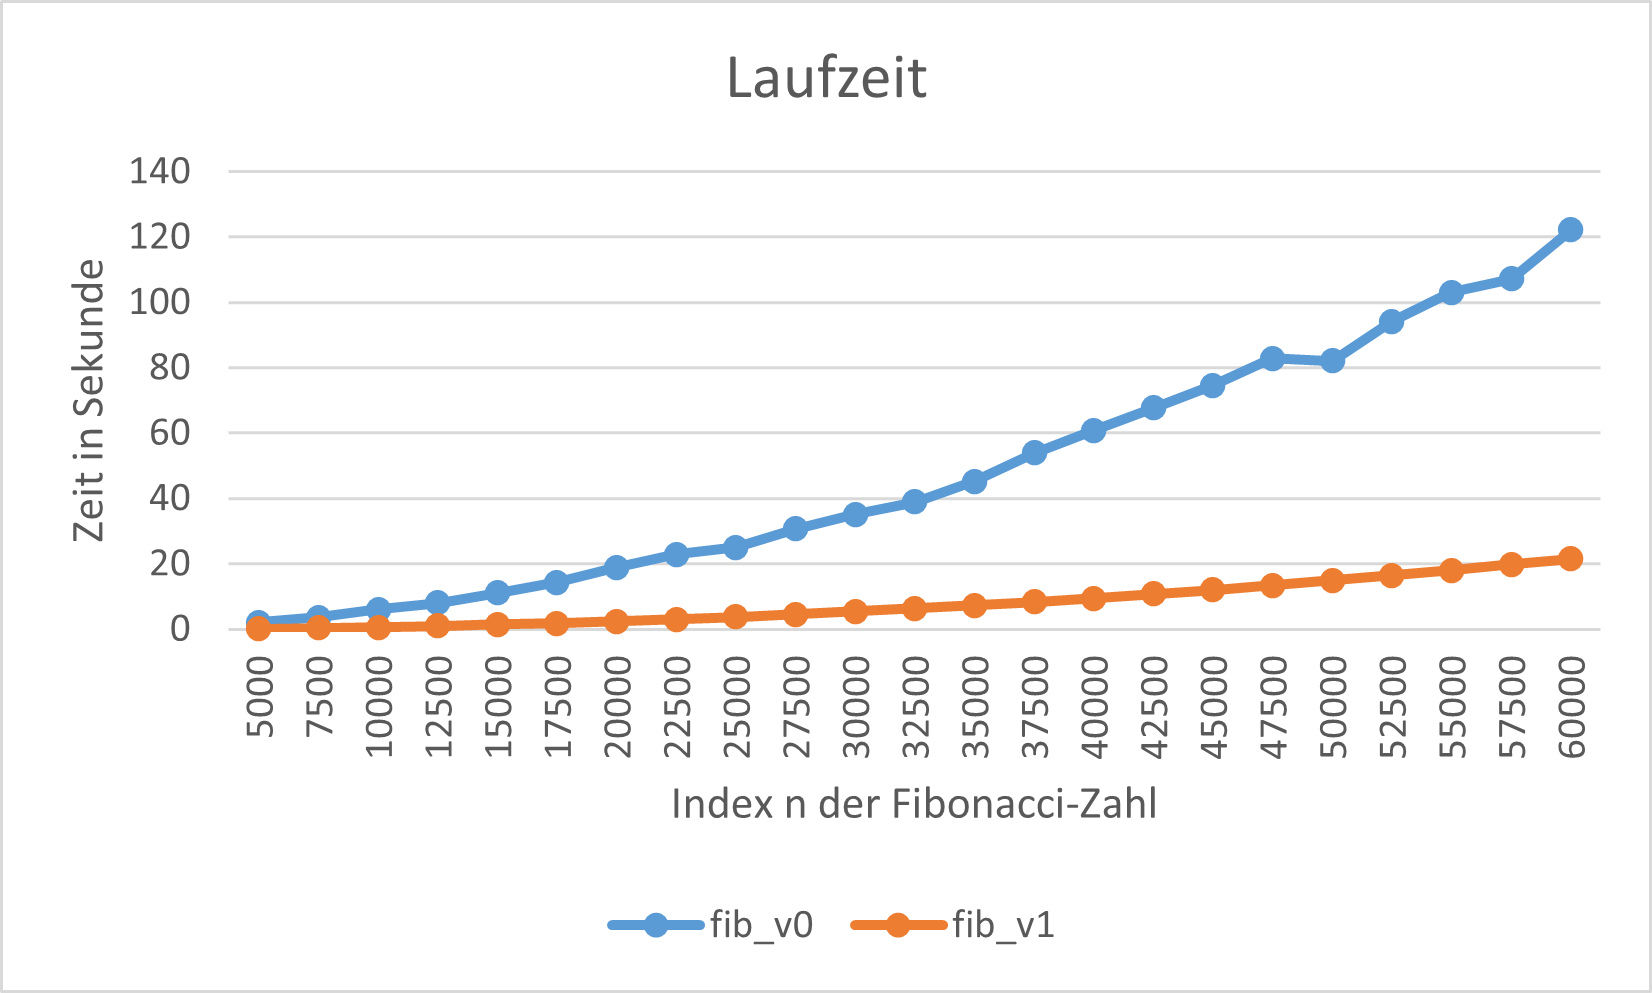
\includegraphics[width=0.8\linewidth]{Laufzeit.png}
    \caption{Laufzeit der fib\_v0 und fib\_v1}
    \label{fig:laufzeit}
\end{figure}
\\Allerdings entspricht die Anzahl der geforderten Additionen nicht der Laufzeit Komplexität der Implementierung. 
Ein wichtiger Grund ist, dass die Länge der Fibonacci-Zahl laut unserer Herleitung linear anwächst. Zugleich hängt die Komplexität der Addition und der Multiplikation laut unserer Implementierung von der Länge der binären Darstellung der berechneten Big-Integer ab. Außerdem wächst die Laufzeit der Multiplikation exponential an. Folglich wächst die Laufzeit der fib\_v1 approximativ quadratisch an. Um die relative Wachstumsrate der beiden Implementierungen zu untersuchen, wird der Quotient der Laufzeit fib\_v0 und fib\_v1 ausgerechnet. Obwohl der Quotient bis der Index $12.500$ stark abnimmt, konvergiert der Quotient mit steigendem Index $n$ gegen eine konstante Zahl.
Zusammenfassend hat fib\_v1 eine ähnliche Laufzeitkomplexität wie fib\_v0 aber deutlich kürzer Laufzeit. Somit stellt unsere Implementierung keine wirkliche Performanzverbesserung dar.

\section{Zusammenfassung und Ausblick}
Zusammenfassend lässt sich sagen, dass in der Theorie durch eine konzeptionelle Optimierung eine größere Performanzverbesserung gewonnen werden kann. Allerdings ist das in der Praxis nicht immer ersichtlich. Es ist stark abhängig von der Gestaltung und Implementierung. Ferner kann man behaupten, dass eine Hardware-Optimierung in manchen Fällen nützlicher als eine Software-Optimierung sein kann. Bei aktuellen Forschungen hat man sogar eine approximative lineare Laufzeit der Multiplikationen zweier riesigen Zahlen erschafft. Solche Bemühungen sind nicht vergeblich, da sie immer ihr Einsatzgebiet in der Praxis finden.
\\Die schnelle Exponentiation hat auch ein umfangreiches Einsatzgebiet. Man kann damit viele Probleme leicht lösen: z.B. die effektive Berechnung von großen Exponenten modulo einer Zahl, die mehrmalige Anwendung einer Permutation, die schnelle Anwendung einer Reihe von geometrischen Operationen auf eine Menge von Punkten und das Finden der Anzahl der Pfade der Länge k in einem Graphen\cite{binaryExponentiation}. Außerdem ist die schnelle Berechnung von Potenzen an sich nützlich in vielen arithmetischen Bereichen.

\newpage
\bibliographystyle{plain}
\bibliography{Ausarbeitung}{}

\end{document}
